\documentclass[paper=a4, fontsize=11pt]{scrartcl} 

\usepackage[T1]{fontenc} 
\usepackage[english]{babel}
\usepackage{amsmath,amsfonts,amsthm}

\usepackage{pstricks}
\usepackage{auto-pst-pdf}

\usepackage{amsmath}
\usepackage{amsfonts}
\usepackage{amssymb}
\usepackage{multicol}
\usepackage{multirow}
\usepackage{hhline}

\usepackage{lipsum}

\usepackage{graphicx}
\usepackage{float}
  \floatplacement{figure}{H}
  \floatplacement{table}{H}
  
\usepackage{sectsty} 
\allsectionsfont{\centering \normalfont\scshape} 

\usepackage{fancyhdr} % Custom headers and footers
\pagestyle{fancyplain} % Makes all pages in the document conform to the custom headers and footers
\fancyhead{} % No page header - if you want one, create it in the same way as the footers below
\fancyfoot[L]{} % Empty left footer
\fancyfoot[C]{} % Empty center footer
\fancyfoot[R]{\thepage} % Page numbering for right footer
\renewcommand{\headrulewidth}{0pt} % Remove header underlines
\renewcommand{\footrulewidth}{0pt} % Remove footer underlines
\setlength{\headheight}{13.6pt} % Customize the height of the header

\usepackage[labelformat=empty]{caption}
\usepackage{color}
\usepackage{listings}
\lstset{ %
language=bash,                % choose the language of the code
basicstyle=\footnotesize,       % the size of the fonts that are used for the code
numbers=left,                   % where to put the line-numbers
numberstyle=\footnotesize,      % the size of the fonts that are used for the line-numbers
stepnumber=1,                   % the step between two line-numbers. If it is 1 each line will be numbered
numbersep=5pt,                  % how far the line-numbers are from the code
backgroundcolor=\color{white},  % choose the background color. You must add \usepackage{color}
showspaces=false,               % show spaces adding particular underscores
showstringspaces=false,         % underline spaces within strings
showtabs=false,                 % show tabs within strings adding particular underscores
frame=single,           % adds a frame around the code
tabsize=2,          % sets default tabsize to 2 spaces
captionpos=b,           % sets the caption-position to bottom
breaklines=true,        % sets automatic line breaking
breakatwhitespace=false,    % sets if automatic breaks should only happen at whitespace
escapeinside={\%*}{*)}          % if you want to add a comment within your code
}
\usepackage{hyperref}


\numberwithin{equation}{section} % Number equations within sections (i.e. 1.1, 1.2, 2.1, 2.2 instead of 1, 2, 3, 4)
\numberwithin{figure}{section} % Number figures within sections (i.e. 1.1, 1.2, 2.1, 2.2 instead of 1, 2, 3, 4)
\numberwithin{table}{section} % Number tables within sections (i.e. 1.1, 1.2, 2.1, 2.2 instead of 1, 2, 3, 4)

\setlength\parindent{0pt} % Removes all indentation from paragraphs - comment this line for an assignment with lots of text

%----------------------------------------------------------------------------------------
%	TITLE SECTION
%----------------------------------------------------------------------------------------

\newcommand{\horrule}[1]{\rule{\linewidth}{#1}} % Create horizontal rule command with 1 argument of height

\title{	
\normalfont \normalsize 
\textsc{Computational Science} \\ [25pt] % Your university, school and/or department name(s)
\horrule{0.5pt} \\[0.2cm] % Thin top horizontal rule
\small Homework - Introduction to Frontiers of Computational Science\\ % The assignment title
%\horrule{2pt} \\[0.5cm] % Thick bottom horizontal rule
}

\author{\small{Ridlo W. Wibowo || 1215011069}} % Your name

\date{\small\today} % Today's date or a custom date


\begin{document}
\maketitle % Print the title

\section{Problem 1}
Solve the following equations:
\begin{equation}
\label{eq:satu}
\frac{d}{dt} x_1(t) = \dot{x}_1 =  \mu(-x_1(t) +   x_2(t)         )
\end{equation}
\begin{equation}
\label{eq:dua}
\frac{d}{dt} x_2(t) = \dot{x}_2 =  \mu( x_1(t) - 2x_2(t) + x_3(t))
\end{equation}
\begin{equation}
\label{eq:tiga}
\frac{d}{dt} x_3(t) = \dot{x}_3 =  \mu(            x_2(t) - x_3(t))
\end{equation}
where $x_i(0) = x^0_i$ ($i=1,2,3$).\\


\textbf{Answer}\\
if we sum all the equations we obtain:
\begin{equation}
\label{eq:jwb1}
\dot{x}_1 + \dot{x}_2 + \dot{x}_3 = 0
\end{equation}
then if we substract \eqref{eq:satu} with \eqref{eq:tiga}, we obtain:
\begin{equation}
\label{eq:jwb2}
\dot{x}_1 - \dot{x}_3 = -\mu(x_1 - x_3)
\end{equation}
also, we can sum \eqref{eq:satu} and \eqref{eq:dua} then substract it with two times \eqref{eq:dua}, and we will get:
\begin{equation}
\label{eq:jwb2}
\dot{x}_1 - 2\dot{x}_2 + \dot{x}_3 = -3 \mu(x_1 - 2x_3 + x_3)
\end{equation}

the solution:
\begin{equation}
\label{eq:sol1}
(x_1 + x_2 + x_3)_{(t)} = (x_1 + x_2 + x_3)_{(0)}
\end{equation}
\begin{equation}
\label{eq:sol2}
(x_1 - x_3)_{(t)} = (x_1 - x_3)_{(0)} e^{-\mu t}
\end{equation}
\begin{equation}
\label{eq:sol3}
(x_1 - 2x_2 + x_3)_{(t)} = (x_1 - 2x_2 + x_3)_{(0)} e^{-3 \mu t}
\end{equation}

if we add two times \eqref{eq:sol1} with \eqref{eq:sol3}:
\begin{equation}
(x_1 + x_3)_{(t)} = \frac{1}{3} x_1^{(0)} ( 2 + e^{-3\mu t}) + \frac{2}{3} x_2^{(0)} ( 1 - e^{-3\mu t}) + \frac{1}{3} x_3^{(0)} (2 + e^{-3\mu t})
\end{equation}
operate with \eqref{eq:sol2}:
\begin{equation}
\label{eq:fin1}
x_1^{(t)} = \frac{1}{6} x_1^{(0)} ( 2 + e^{-3\mu t} + e^{-\mu t}) + \frac{1}{3} x_2^{(0)} ( 1 - e^{-3\mu t}) + \frac{1}{6} x_3^{(0)} ( 2 + e^{-3\mu t} - e^{-\mu t})
\end{equation}
\begin{equation}
\label{eq:fin2}
x_3^{(t)} = \frac{1}{6} x_1^{(0)} ( 2 + e^{-3\mu t} - e^{-\mu t}) + \frac{1}{3} x_2^{(0)} ( 1 - e^{-3\mu t}) + \frac{1}{6} x_3^{(0)} ( 2 + e^{-3\mu t} + e^{-\mu t})
\end{equation}
if we substract \eqref{eq:sol1} with \eqref{eq:sol3}:
\begin{equation}
\label{eq:fin3}
x_2^{(t)} = \frac{1}{3} x_1^{(0)} ( 1 - e^{-3\mu t}) + \frac{1}{3} x_2^{(0)} ( 1 + 2e^{-3\mu t}) + \frac{1}{3} x_3^{(0)} ( 1 - e^{-3\mu t})
\end{equation}

so we get the solutions for this problem in equation \eqref{eq:fin1}, \eqref{eq:fin2}, and \eqref{eq:fin3}. We also can use eigenvalue problem to get the same result.

%\begin{figure}
%	\centering
%	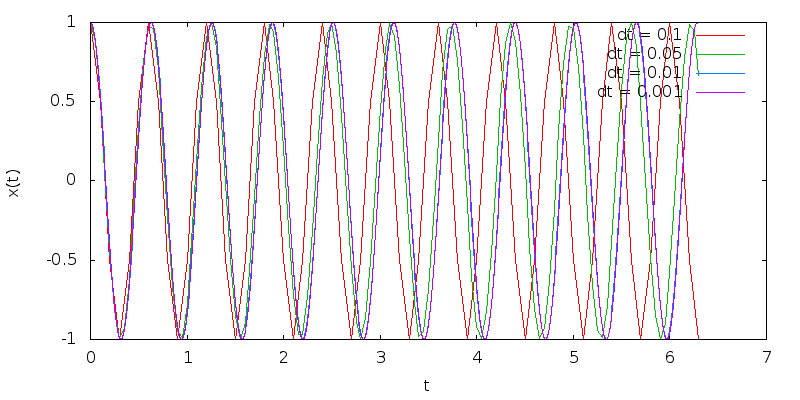
\includegraphics[width=0.8\textwidth]{verlet2.png}
%	\caption{Comparison of the result from Verlet algorthm using different $\Delta t$.}
%\end{figure}

\newpage
\section{Problem 2}
Check if $\begin{pmatrix} 1 \\ 1 \\ 1\end{pmatrix}$, $\begin{pmatrix} 1 \\ 0 \\ -1\end{pmatrix}$, and $\begin{pmatrix} 1 \\ -2 \\ 1\end{pmatrix}$ are orthogonal to each others. Normalize and check the unitary condition.\\


\textbf{Answer}:\\
for orthogonality we can use dot product to each pair of vector:
$v_{i} \cdot v_{j} = 0$ for $i \neq j$, easily we can prove that all combination resulting zero dot product. For example:\\
$ v_1 \cdot v_2 = \begin{pmatrix} 1 \\ 1 \\ 1 \end{pmatrix} \cdot \begin{pmatrix} 1 \\ 0 \\ -1 \end{pmatrix} = 1\cdot 1 + 1 \cdot 0 + 1 \cdot -1 = 0 $\\

Normalize vector would be $(e_1, e_2, e_3)$:\\
$\frac{1}{\sqrt{3}} \begin{pmatrix} 1 \\ 1 \\ 1 \end{pmatrix}$, $\frac{1}{\sqrt{2}} \begin{pmatrix} 1 \\ 0 \\ -1 \end{pmatrix}$, and $\frac{1}{\sqrt{6}} \begin{pmatrix} 1 \\ -2 \\ 1 \end{pmatrix}$

Checking unitary relation\\
$Q = \begin{pmatrix} \frac{1}{\sqrt{3}} & \frac{1}{\sqrt{2}} & \frac{1}{\sqrt{6}} \\ 
\frac{1}{\sqrt{3}} & 0 & \frac{-2}{\sqrt{6}} \\
\frac{1}{\sqrt{3}} & \frac{-1}{\sqrt{2}} & \frac{1}{\sqrt{6}}
\end{pmatrix}$\\


if we inverse it using $Q^{-1} = \frac{1}{\det(Q)} (adj(Q))$, this matrix will become:\\


$Q^{-1} = 
\begin{pmatrix} 
\frac{1}{\sqrt{3}} & \frac{1}{\sqrt{3}} & \frac{1}{\sqrt{3}}\\ 
\frac{1}{\sqrt{2}} & 0 & \frac{-1}{\sqrt{2}} \\
\frac{1}{\sqrt{6}} & \frac{-2}{\sqrt{6}} & \frac{1}{\sqrt{6}}
\end{pmatrix}$\\


and the unitary relation is proven $Q^{-1} = Q^{T}$


\begin{postscript}
\psset{fillstyle=solid}
\psscalebox{0.75}{%
\begin{pspicture}(-5.25,-5.25)(5.25,5.25)%
  \pscircle*[linecolor=cyan]{5}
  \psgrid[subgriddiv=0,gridcolor=lightgray,gridlabels=0pt]
  \Huge\sffamily\bfseries
  \rput(-4.5,4.5){A} \rput(4.5,4.5){B}
  \rput(-4.5,-4.5){C}\rput(4.5,-4.5){D}
  \rput(0,0){auto-pst-pdf}
  \rmfamily
  \rput(0,-3.8){PSTricks}
  \rput(0,3.8){\LaTeX}
\end{pspicture}}
\end{postscript}

\scalebox{1} % Change this value to rescale the drawing.
{
\begin{pspicture}(0,-2.69)(5.38,2.69)
\psframe[linewidth=0.04,dimen=outer](5.38,2.69)(0.0,-2.69)
\psframe[linewidth=0.04,dimen=outer](4.34,1.53)(1.2,-1.61)
\psframe[linewidth=0.04,dimen=outer](2.18,1.31)(1.48,0.61)
\psframe[linewidth=0.04,dimen=outer](3.16,-0.79)(2.48,-1.47)
\end{pspicture} 
}

\end{document}